\chapter{Software}
\label{methods}
\section{Computefarm}
\label{computefarm}
\subsection{Inspiration}
As discussed in Chapter \ref{background}, global optimization solvers depend on the computational time. They also depend on fault tolerance of the objective function and resource consumption. In the event that a black box function takes a long computational time, most global optimization software offer a parallel option. However, this is not beneficial when the function evaluation consumes a lot of resources in order to run the objective function. In this situation multiple function evaluations are run simultaneously, increasing the amount of resources needed by a multiple of the number of objective functions in play. When this occurs, the demand for resources from the optimization becomes higher than the machine can provide and results in what is known as \textit{resource contention}. 


This is one of the motivations behind Computefarm, a software application that parallelizes global optimization solvers by distributing function evaluations to client computers. Distributing the evaluations out to client computers minimizes resource contention and allows for a number of search-space points to be evaluated simultaneously. Computefarm also handles failures in the client machines. If a client disconnects or fails to run the function evaluation, Computefarm resassigns the evaluation to another client. By contrast, when a single machine faces a failure on its own, the entire optimization process is interrupted and needs to be restarted. By using Computefarm for global optimization algorithms, the user is able to run the program in parallel, avoid high resource contention and obtain fault-tolerance in the function evaluations.   
\clearpage 
\subsection{Requirements}
Computefarm is a distributed system that delegates tasks to multiple client computers. In the case of global optimization, a server distributes function evaluations to client computers. Three things are required to minimize the overhead of using Computefarm. These are:
\begin{itemize}
    \item the port number for socket connection (user-provided),
    \item the script name of the objective function being run (also user-provided), and
    \item the list of population points at which to evaluate the objective function on client machines (global optimization algorithm-provided).
\end{itemize}
The first two items are passed into the solver and subsequently passed along to Computefarm for the initialization phase. The last item is passed in by the algorithm according to the metric it uses to determine which points in the domain of the objective function should be evaluated at each iteration step.  
\subsection{Structure}
 The implementation of Computefarm is based on the client-server model, meaning that the software farms unused or accessible client machines to wait upon directives of the server machine. For global optimization specifically, the server delegates points in the search space for the client computers to evaluate a black-box function. The clients return the results to the server machine, and wait for further positions to evaluate. The server then provides a list of results to the global optimization solver from each point of evaluation. 


In the case of a failure the server will receive a disconnect from the client machine, and return that machine's search-space position to the queue of positions pending evaluation. The server will later provide that position to a client waiting on a new point to evaluate. This ensures fault tolerance in the Computefarm software because the global optimization solver does not need to restart if a client computer fails. 


An extra step is taken in Computefarm whereby client machines are reawakened to ensure the maximum number of machines are available to the server. 
  Figure \ref{fig:computefarm} shows the flow of a global optimization algorithm using Computefarm. 
\clearpage
\begin{figure}[h!]
    \centering
    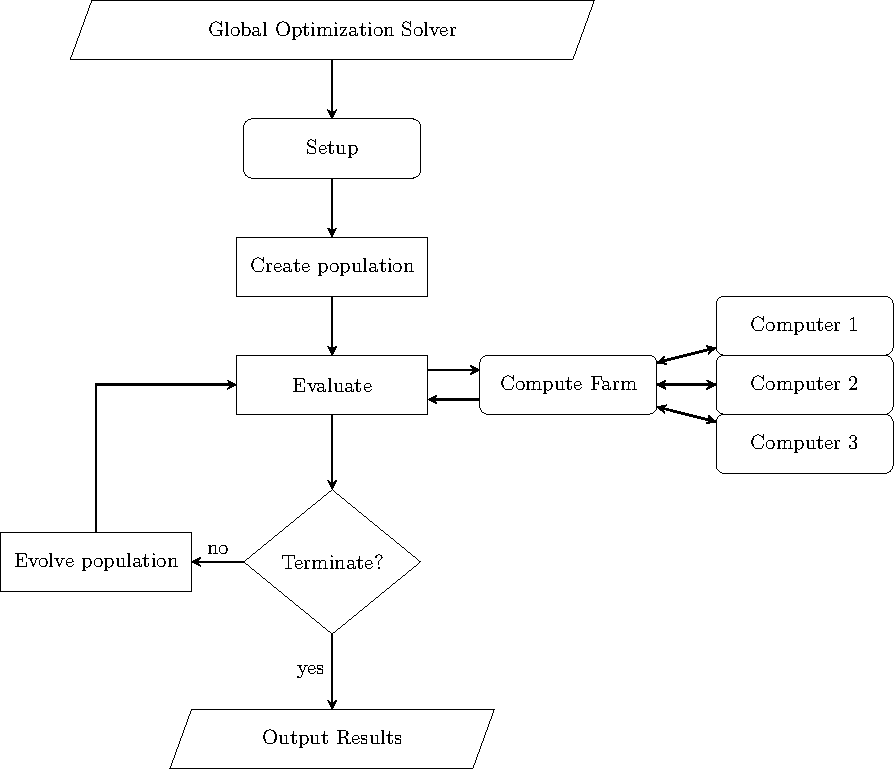
\includegraphics[width=10cm,height=15cm]{chapters/chapter_3_Software/flowchart.pdf}
    \caption{Process of a global optimization algorithm using Computefarm}
    \label{fig:computefarm}
\end{figure}
Computefarm will take a list of population points and distribute them out to various client computers, which will return a list of results to the global optimization algorithm to further proceed in the process. In this thesis we implement a Particle Swarm Optimization (PSO) algorithm that leverages Computefarm to solve the problems described in Chapter \ref{applications}. The original PSO algorithm is described in Alg. \ref{algorithmPSO} and the Computefarm version in Alg. \ref{CFPSO}

\begin{algorithm}[H]
  \begin{algorithmic}[2]

      \State \textbf{initialize} Computefarm \Comment{initializes the setup of the software}
    \For{each particle i}
        \State \textbf{initialization} $x_i$, $v_i$, $xbest_i$ \Comment{random value for $x_i$ and $v_i$}
        $xbest_i \gets xbest_i$
    \EndFor
    \State \textbf{Evaluate} Computefarm(X) \Comment{evaluate the list of points X using Computefarm}
    \For{each particle i}
        \State \textbf{Update} $xbest_i$ \Comment{update if $f(x_i) < f(xbest_i)$}
    \EndFor
    \While{not termination condition}
        \For{each particle i}
            \State \textbf{update} xglobal \Comment{update if $f(xglobal) < f(xbest_i)$}
            \State \textbf{calculate} $v_i$ \Comment{using one of the PSO velocity equations}
            \State $x_i = x_i + v_i$
        \EndFor
        \State \textbf{Evaluate} Computefarm(X)
        \For{each particle i}
            \State \textbf{update} $xbest_i$
        \EndFor
    \EndWhile
  \end{algorithmic}
\caption{Computefarm Particle Swarm Optimization}
\label{CFPSO}
\end{algorithm}
 
This algorithm is applied in the PSO variants in the software \textit{pythOPT}, a problem-solving environment, creating a distributed PSO version called Computefarm Particle Swarm Optimization (CFPSO).

To further understand the implementation steps taken in Computefarm, Figure \ref{fig:implementation} shows the overall design of the distributed system. 
\clearpage
\begin{figure}[h!]
    \centering
    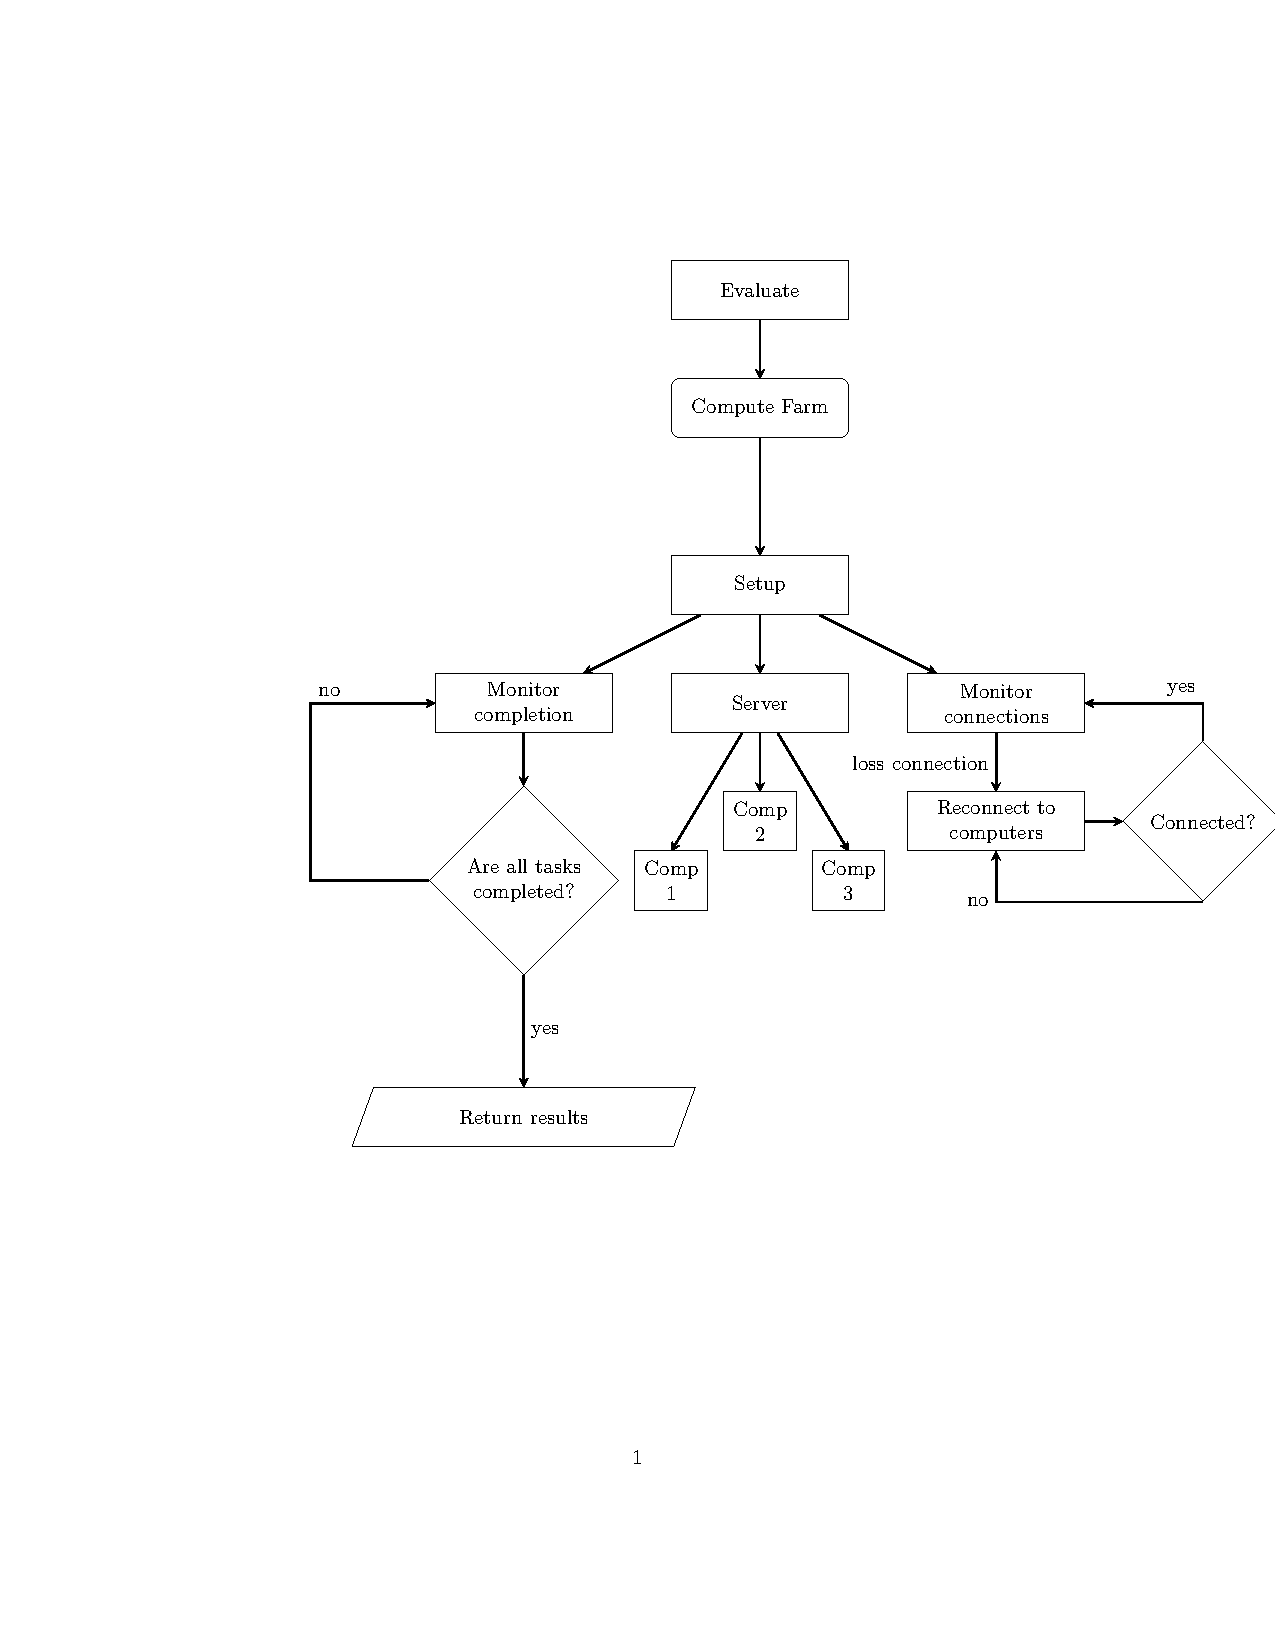
\includegraphics[width=10cm,height=15cm]{chapters/chapter_3_Software/flowchart2.pdf}
    \caption{Process of a global optimization algorithm using Computefarm}
    \label{fig:implementation}
\end{figure}

During the setup phase of Computefarm, three POSSIX \textit{threads} are used to run the following functions:
\begin{itemize}
    \item Monitor Completion,
    \item Server, and
    \item Monitor Connections. 
\end{itemize}

Threads are used in this software because of their shared memory properties, which allow a form of message passing in the program. Each thread function takes care of a single process that monitors a list to determine further actions. The lists that are shared in memory between the three threads are the medium for message passing in the program. 

The Monitor Completion function takes care of monitoring whether all tasks are completed before returning the results to the solver. The Server function creates a TCP socket and binds to any client computers communicating on the same port. TCP sockets were chosen because of their reliable connection handling. Threads are generated for each connected client to allow for concurrency in the server system. Each connection is taken care of by a connection handler that will assign itself to a client machine by receiving the hostname of that machine. Once this is obtained, the connection handler will change an client-assigned flag for that machine from zero to one. Afterward, it will continue to monitor the particle list that contains the particle information structure, which includes: 

\begin{itemize}
    \item particle number,
    \item particle position,
    \item function value,
    \item length of position, 
    \item assigned flag, and
    \item completion flag.
\end{itemize}
If any particle is not assigned to a connection handler then the connection handler will change the assigned flag from zero to one, indicating that it has been assigned. To ensure multiple connection handlers do not assign themselves the same particle, \textit{mutexs} are used to ensure mutual exclusion. Once a connection handler has assigned itself a particle, it will then transmit the particle position information to the client computer using the TCP socket. Because this portion of the program is written in the programming language C, the particle position array length is also stored and sent to the client computer. The connection handler will then wait to receive a message from the client. This message will contain the resulting function evaluation. The connection handler will then store the function value for the specific particle and change the finished flag from zero to one. In the case of a client disconnect, the connection handler will de-assign itself from the particle by reversing the client-assigned flag to zero, and exit. The work flow of the connection handler is displayed in the following Figure \ref{fig:connection handler}.

\begin{figure}[h!]
    \centering
    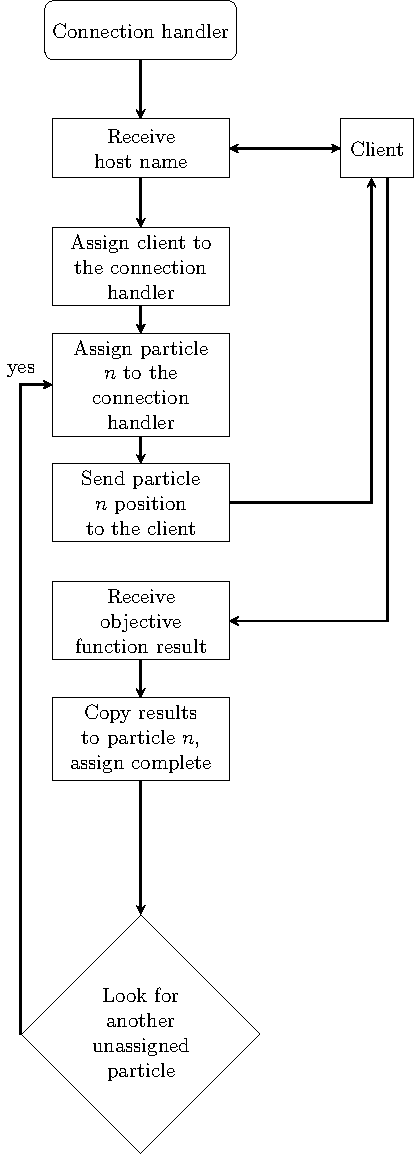
\includegraphics[width=8cm,height=10cm]{chapters/chapter_3_Software/connection_handler.pdf}
    \caption{Computefarm connection handler work flow}
    \label{fig:connection handler}
\end{figure}

The Monitor Connection function awakens client machines to run the client script to connect to the server and monitor any machines that disconnect. When machines disconnect, a separate thread function, Reawaken Clients, will attempt to awaken any known disconnected machines every $N$ minutes (with the default set to ten minutes). This ensures the maximum number of client machines will be connected to the server every $N$ minutes from start up. Disconnected machines are determined by the assigned flag in the client structure containing the host name of the machine. When the assigned flag is zero, the Reawaken Clients function will attempt to awaken that client machine. 


In the second phase of Computefarm, the Server and Monitor Connections threads will be kept alive while the Monitor Completion function is called by the solver. The Monitor Completion function will re-initialize the particle list with new positions and reset all other information on the particle. The process of the Server and Monitor Connections will continously run to complete all function evaluations. Once every particle is evaluated, the Monitor Completion will return the results to the solver. This phase will be repeated multiple times before the final phase, where the solver completes its optimization process and terminates. To ensure no leakage of memory or zombie threads, a termination function will be called by the solver to terminate all threads and processes running within Computefarm. 


\section{Optimization Database}
\label{database}
\subsection{Inspiration}
The Optimization Database is used to deal with various challenges that emerge in the global optimization process. One set of challenges has to do with monitoring the optimization to determine whether the problem is solved. Because global optimization solvers run until a termination condition is satisfied, a solution could be found sooner than later. A standard method of monitoring the optimization process involves having the best value at each iteration printed or saved in a log file. This method can be unreliable, however, in the event that the file cannot be saved or if printed values are lost due to a failure. Moreover, sorting through printed information or files is a lengthy process that may require extra code. One way to address these challenges is to use a database to store values in accordance with a policy. In the optimization database there are three policies the user can chose from:
\begin{itemize}
    \item best value, 
    \item every evaluation, or
    \item evert $n$th evaluation.
\end{itemize}
The database will store values based on the policy chosen at each evaluation. Adding a value to the database ensures the transaction is completed. This is because of the following feature: if the transaction fails, an error is reported and two attempts are made to reconnect and insert the data. If these additional attempts are unsuccessful, it will send an alert to the user and continue the optimization process. 

 
Some situations that require monitoring include:
\begin{itemize}
    \item premature convergence, 
    \item performance testing, and
    \item obtaining results.
\end{itemize}

Another challenge of global optimization is obtaining $N$ best solutions. Because global optimization is implemented to solve for the global minimum, it is unusual to have a solver that returns the $N$ best global solutions. The Optimization Database is therefore used to sort through the data to obtain the $N$ best solutions that the solver explored. This is shown to be useful in Chapter \ref{rational design} with respect to the crystal structure prediction problem. The metastable structures of crystals are of particular interest because of their properties; diamond, for example, is a metastable structure of carbon with the stable structure being graphite. In a global optimization, graphite is the global minimum because it has the lowest total energy. Diamond, with the second lowest total energy, has the property of being very hard and is used in multiple research experiments to define hardness in relation to other stuctures. The Optimization Database is used to obtain the $N$ lowest energy crystal structures for various compounds. 


Yet another data-storing problem for global optimization is obtaining extra information on the objective function. Extra information may include:
\begin{itemize}
    \item information on the data (e.g. the symmetry group of a predicted crystal structure), or
    \item sorting information on various instances (e.g. the time duration to correct for errors in a quantum component, as discussed in Chapter \ref{qubit}).
\end{itemize}
The Optimization Database is used to store information on the optimization of the objective function. The database allows for user flexibility with respect to storage policies for extra information, enabling easier and more reliable data collection on the global optimization process. 

\subsection{Requirements}

We maintain a database that stores the status of optimization runs. This database can be used to store both local and global solver statuses, but in this thesis we restrict it to global. The database is primarily operated by a single user to keep track of the progress of a solver on a problem of interest. The primary information needed is:
\begin{itemize}
    \item PostgreSQL database information, 
    \item problem name, and 
    \item global optimization settings.
\end{itemize}

\subsection{Schema}

The Optimization Database is implemented for users with no prior knowledge of databases. If the user does not already have a local or remote database set up, the software will create a local PostgreSQL database. It will then automatically produce two tables, for settings and problem. The former  stores information about the settings used for the global optimization, with the following default columns:
\begin{itemize}
    \item global optimization method,
    \item lower bound,
    \item upper bound,
    \item seed, and
    \item note on simulation. 
\end{itemize}
Columns that are included and maintained by the database are:
\begin{itemize}
    \item primary key ID,
    \item status, and 
    \item check-in time. 
\end{itemize}
The primary key is used to associate any instance of the problem that will be storing its data in the problem table. The status column is updated by the software to keep tabs on whether a simulation is running. Whenever the database is updated or inserted into, the check-in time will be automatically updated to the current time. The check-in time can later be used to determine whether the simulation has been running for the past $N$ hours. These features of the software, in combination with an automatic email component, allow the user to be regularly notified regarding the status and results of the optimization. 


The problem table is used to record the data on the objective function. By default, it stores: 
\begin{itemize}
    \item foreign key ID,
    \item $x$ position,
    \item $f$ (function evaluation result),
    \item evaluation number, and
    \item insertion time.
\end{itemize}
The user can also opt for additional columns to store other data about the objective function. As previously mentioned, this can be utilized for faster sorting methods between instances or properties of the simulation. 

Figure \ref{fig:database schema} represents the database schema used by the software where one settings table has multiple instances of problem tables. 


\begin{figure}[!h]
    \centering
    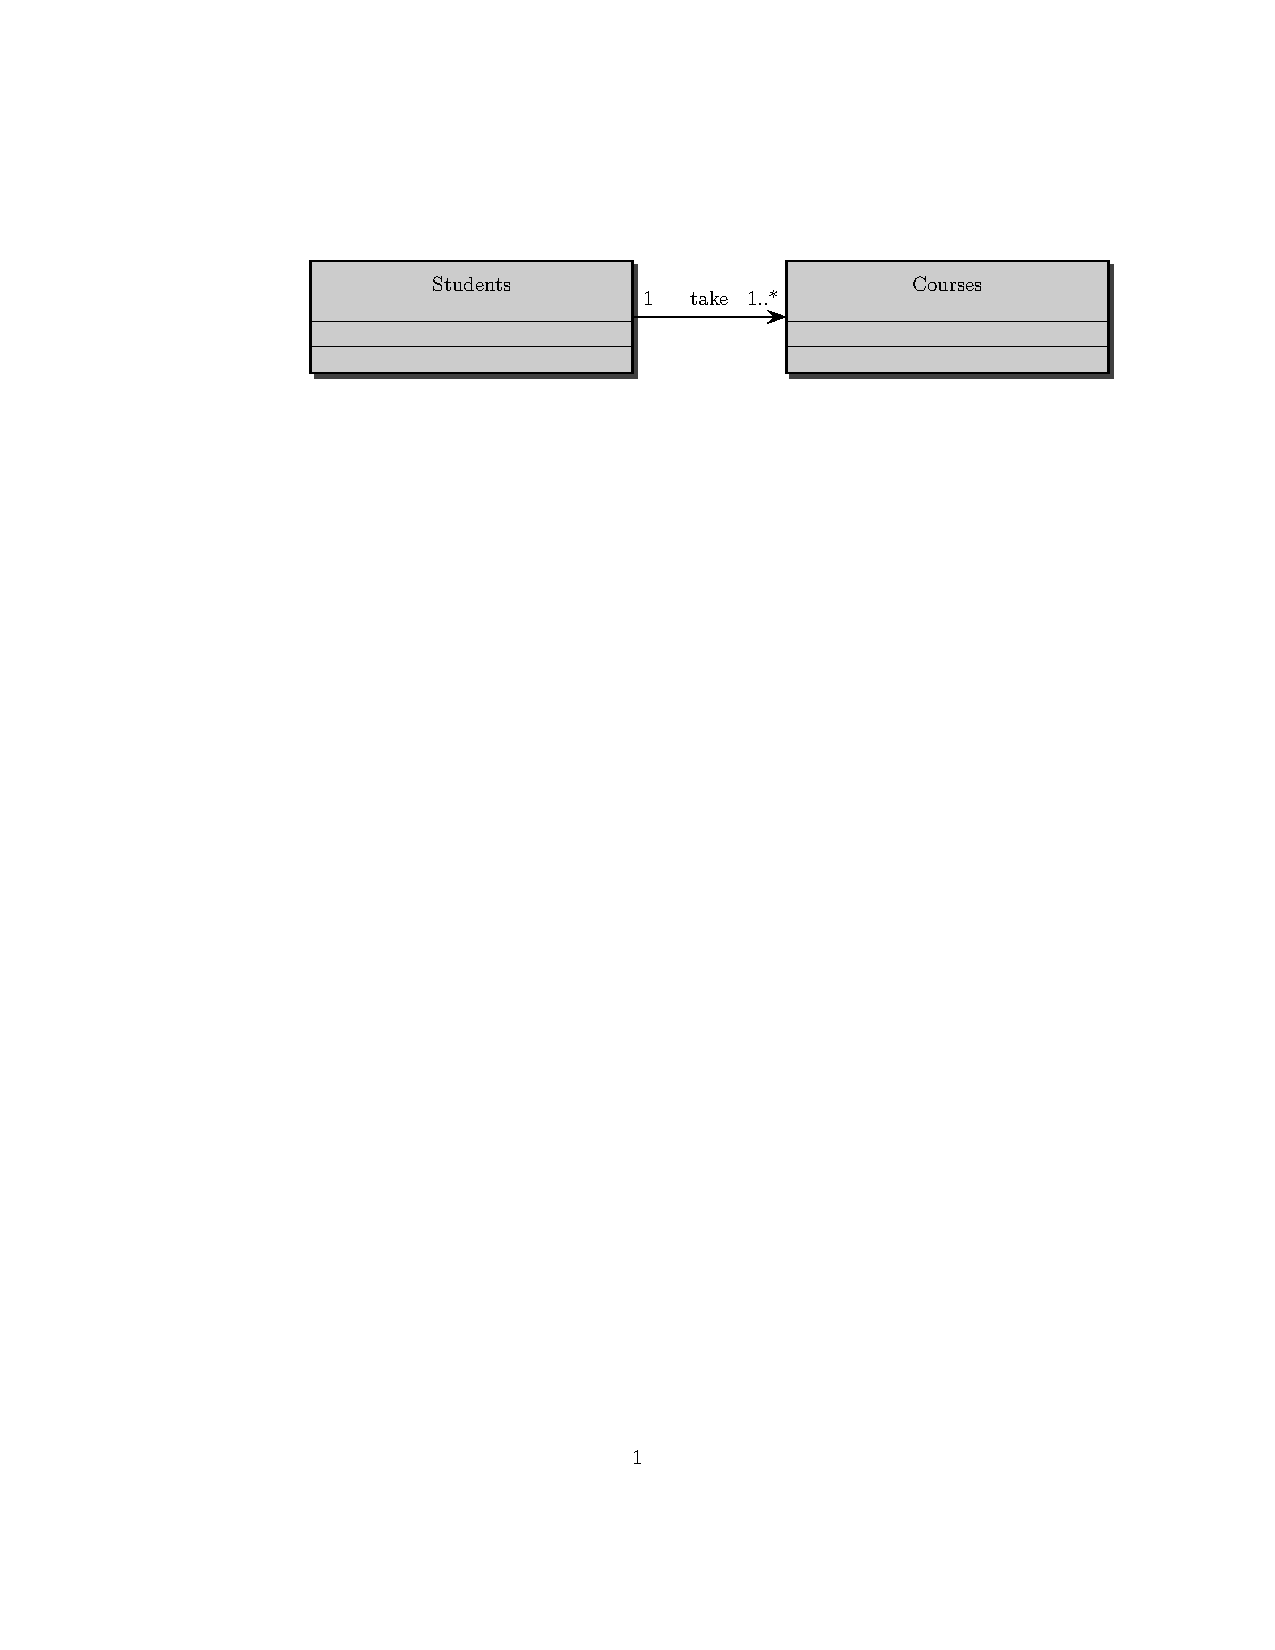
\includegraphics[width=5cm]{chapters/chapter_3_Software/database_schema.pdf}
    \caption{Optimization Database schema}
    \label{fig:database schema}
\end{figure}




